\documentclass[runningheads,a4paper]{llncs}
\usepackage{amssymb}
\setcounter{tocdepth}{3}
\usepackage{graphicx}
\usepackage{listings}
\usepackage{subfigure}
\usepackage{url}
\usepackage{cite}
\urldef{\mailsa}\path|{jbrunelle, mln}@cs.odu.edu|    
\newcommand{\keywords}[1]{\par\addvspace\baselineskip
\noindent\keywordname\enspace\ignorespaces#1}
\usepackage{colortbl}
\usepackage{alltt}

%\parskip 0pt 
\begin{document}

\mainmatter

\title{Evaluating the SiteStory Transactional Web Archive With the ApacheBench Tool}

\author{Justin F. Brunelle\inst{1,2} \and Michael L. Nelson\inst{2} \and Lyudmila Balakireva\inst{3} \and Robert Sanderson\inst{3} \and Herbert Van de Sompel\inst{3}
}

\institute{The MITRE Corporation, Hampton, VA 23666\\
\email{jbrunelle@mitre.org}
\and
Old Dominion University, Department of Computer Science,
Norfolk VA, 23529\\
\email{\{jbrunelle, mln\}@cs.odu.edu}
\and
Los Alamos National Laboratory, 
Los Alamos, NM 87544\\
\email{\{ludab, rsanderson, herbertv\}@lanl.gov}
}


%
% NB: a more complex sample for affiliations and the mapping to the
% corresponding authors can be found in the file "llncs.dem"
% (search for the string "\mainmatter" where a contribution starts).
% "llncs.dem" accompanies the document class "llncs.cls".
%

\maketitle


\begin{abstract}
\sloppy Conventional Web archives are created by periodically crawling a Web
site and archiving the responses from the Web server.  Although easy to
implement and commonly deployed, this form of archiving typically misses
updates and  may not be suitable for all preservation scenarios, for
example a site that is required (perhaps for records compliance) to keep
a copy of all pages it has served.  In contrast, transactional archives
work in conjunction with a Web server to record all content that has
been served.  Los Alamos National Laboratory has developed SiteStory, an
open-source transactional archive written in Java that
runs on Apache Web servers, provides a Memento compatible access
interface, and WARC file export features. We used Apache's ApacheBench
utility on a pre-release version of SiteStory to measure response time and
content delivery time in different environments. 
The performance tests were designed to determine the
feasibility of SiteStory as a production-level solution for high
fidelity automatic Web archiving.  We found that SiteStory does not
significantly affect content server performance when it is performing
transactional archiving.  Content server performance slows from 0.076
seconds to 0.086 seconds per Web page access when the content server is
under load, and from 0.15 seconds to 0.21 seconds when the resource has
many embedded and changing resources.\fussy

\keywords{Web Archiving, Digital Preservation}
\end{abstract}



%Transactional Archiving solutions capture each different representation of Web resources delivered by a content server upon requested access. Such utilities reside on a Web server, and capture content as its delivered. Since a transactional Web archive sits between the content server and the content recipient, it is important to understand how such a solution will affect the server's ability to deliver content. Specifically, content delivery time is important -- a transactional Web archive is no use if it cripples the server's ability to deliver content in a timely manner. Los Alamos National Laboratory (LANL) has developed an open-source transactional Web archiver called SiteStory. SiteStory is a Java solution that runs on Apache Web servers, provides a Memento compatible access interface, and WARC file export features. SiteStory was stress-tested to measure response time and content delivery time in different environments and on different machines. The performance tests were designed to determine the feasibility of  SiteStory as a production-level solution for high fidelity automatic Web archiving. This work finds that  SiteStory does not significantly affect content server performance when it is performing transactional archiving. Content server performance slows from 0.076 seconds to 0.086 seconds per Web page access when the content server is under load, and from 0.15 seconds to 0.21 seconds when the resource has many embedded and changing resources. 

\section{Introduction}
\label{intro}
\vskip -3mm
Web archiving is an important aspect of cultural, historical, governmental, and institutional memory. The cost of capturing Web-native content for storage and archiving varies and is dependent upon several factors. The cost of manual Web archiving has prompted research into automated methods of digital resource capture. The traditional method of automatic capture is the Web crawler, but recent migrations toward more personalized and dynamic resources have rendered crawlers ineffective at high-fidelity capture in certain situations. For example, a crawler cannot capture every representation of a resource that is customized for each user. Transactional archiving can, in some instances, provide an automatic archiving solution to this problem.

\subsection{Transactional Archiving}
\label{ta}
\vskip -3mm
%Transactional archiving is a method of automatically capturing digital content. Transactional Web archives (TWAs) capture content when it is requested by and delivered to a user or user agent. TWAs are software solutions that are installed on a content server. This software listens for requests for content residing on the local content server by a user or other agent. These requests mostly take the form of HTTP GET requests (seen in Figure \ref{get}). The traditional method of requesting content from a server begins with the client-initiated HTTP GET request for a resource R to the server. The GET request is received by the server, and the content (if available) for resource R's representation is returned to the requesting client with an accompanying HTTP 200 status code in the response reader. As the content is returned to the requesting agent, SiteStory software makes and archives a copy of the representation. The archived copy is only stored if the representation is a new, never seen before representation. This effectively stores each different representation of a resource that a user sees. 

The purpose of a transactional archive (TA) is to archive every
representation of a resource that a Web server disseminates.  A client
does an HTTP GET on a URI and the Web server returns the representation
of the resource at that time.  At dissemination time, it is the
responsibility of TA software to send to an archive the representation sent to the client.
  In this way, \emph{all}
representations returned by the Web server can be archived.  If storing
all served representations is costly (e.g., a high-traffic site with
slowly changing resources), it is possible to optimize a TA in a
variety of ways: store only unique representations, store every
n$^{th}$ representation, etc.


\begin{figure}[t]
\begin{center}
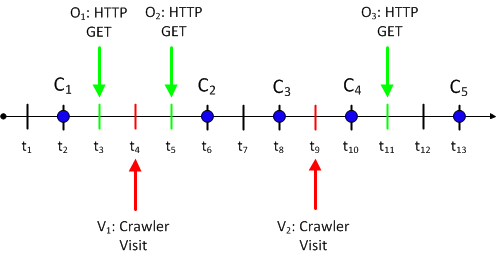
\includegraphics[width=1\textwidth]{change_timeline_crawler.png}
\caption{User and crawler accesses control the archival interval, capturing each returned representation.}
\vskip -3mm
\label{timeline}
\end{center}
\end{figure}


Figure \ref{timeline} provides a visual representation of a typical scenario where a page \emph{P} is both changed and access at irregular intervals. This scenario assumes an arbitrary page that will be called \emph{P} changes at inconsistent intervals. This timeline shows page \emph{P} changes at points $C_{1}$, $C_{2}$, $C_{3}$, $C_{4}$, and $C_{5}$ at times $t_{2}$, $t_{6}$, $t_{8}$, $t_{10}$, and $t_{13}$, respectively. A user makes a request for \emph{P} at points $O_{1}$, $O_{2}$, and $O_{3}$ at times $t_{3}$, $t_{5}$, and $t_{11}$, respectively. A Web crawler (that captures representations for storage in a Web archive) visits \emph{P} at points $V_{1}$ and $V_{2}$ at times $t_{4}$ and $t_{9}$, respectively. 

Since $O_{1}$ occurs after change $C_{1}$, an archived copy of $C_{1}$
is made by the TA. 
%When $O_{2}$ is made, \emph{P} has not changed since
%$O_{1}$ and therefore, an archived copy is not made since one already
%exists. 
The Web crawler visits $V_{1}$ captures $C_{1}$, and makes a
copy in the Web archive.  In servicing $V_{1}$ or $O_{1}$, an unoptimized TA will store
another copy of $C_{1}$ at $t_{4}$ and an optimized TA could detect that no 
change has occurred and not store another copy of $C_{1}$.

Change $C_{2}$ occurs at time $t_{6}$, and $C_{3}$ occurs at time
$t_{8}$. There was no access to \emph{P} between $t_{6}$ and $t_{8}$,
which means $C_{2}$ is lost -- an archived copy exists in neither the
TA nor the Web crawler's archive. However, the argument can be made
that if no entity observed the change, should it be archived?
Change $C_{3}$ occurs and the representation of \emph{P} is archived during the crawler's visit
$V_{2}$, and the TA will also archive $C_{3}$.  After $C_{4}$, a user
accessed \emph{P} at $O_{3}$ creating an archived copy of $C_{4}$ in
the TA.  

In the scenario depicted in Figure \ref{timeline}, the TA will have
changes {$C_{1}$, $C_{3}$, $C_{4}$}, and a conventional archive will
only have {$C_{1}$, $C_{3}$}.  Change $C_{2}$ was never served to any
client (human or crawler) and is thus not archived by either system.
Change $C_{5}$ will be captured by the TA when \emph{P} is accessed
next.

%The example in Figure \ref{timeline} demonstrates SiteStory's ability to capture a single version of each user-observed version of a page, but does not capture versions unseen by users.

\subsection{SiteStory}
\vskip -3mm
\sloppy Los Alamos National Laboratory has developed SiteStory\footnote{\url{http://mementoWeb.github.com/SiteStory/}}, an open-source transactional Web archive.  
%Figure \ref{twa} illustrates the components and process of SiteStory.  
First, mod\_sitestory is installed on the Apache server that contains the content to be archived.  When the Apache server builds the response for the requesting client, mod\_sitestory sends a copy of the response to the SiteStory Web archive, which is deployed as a separate service.  This Web archive then provides Memento-based access to the content served by the Apache server with mod\_sitestory installed, and the SiteStory Web archive is discoverable from the Apache Web server using standard Memento conventions (see Section 4 of \cite{memento:rfc}).

Sending a copy of the HTTP response to the archive is an additional task for the Apache Web server, and this task must not come at too great a performance penalty to the Web server.  The goal of this study is to quantify the additional load mod\_sitestory places on the Apache Web server to be archived.\fussy


\begin{figure}[t]
\begin{center}
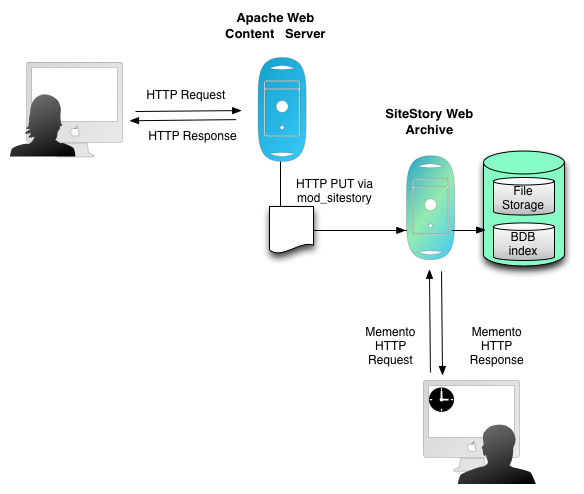
\includegraphics[width=0.5\textwidth]{twa_sitestory.png}
\caption{SiteStory consists of two parts: mod\_sitestory which is installed on the Apache server to be archived, and the transactional archive itself.  Image taken from the SiteStory GitHub at \texttt{http://mementoWeb.github.com/SiteStory/}.}
\vskip -3mm
\label{twa}
\end{center}
\end{figure}



%A delay is incurred on the delivery of content from the server to the requesting agent due to the additional process of the transactional Web archive's need to analyze content as it is returned by the content server. A delay that is too lengthy renders a server unable to function. It is necessary to measure the delay introduced to the request-response transaction. This measures the effect of a beta version of SiteStory on the performance of a content server to ensure that this TWA system does not cripple a Web server when running.


%%%%TPDL 2013 COMMENT
%\subsection{Organization and Purpose}
%\label{organization}
%This Technical Report details the work performed with SiteStory, and the results of the performance tests and benchmarking performed as part of a feasibility study. 
%The rest if this Technical Report is organized as follows: Section \ref{priorwork} discusses the contributions of prior research efforts. Section \ref{experiment} discusses the experiment design and execution. Section \ref{results} details the results and findings of the experiment. Finally, Section \ref{conclusion} summarizes the findings and impacts of this Technical Report, and outlines the upcoming extensions of this work. 

\section{Prior Work}
\label{priorwork}
\vskip -3mm
Extensive research has been done to determine how Web documents change on the Web.  Studies of ``wild'' pages (such as Cho's work with crawlers \cite{cho2000evolution} or Olston's work in recrawl scheduling \cite{olston2008recrawl}) have shown that pages change extremely frequently.  
%Figure \ref{olston} (taken from Olston's paper) visually shows the ephemeral nature of information contained within a Web page.  In this figure, one can see that not only do pages change very frequently, but one can see that pages change in different ways.  In this figure, Page A has small sections of content that change rapidly.  This behavior is called ``churn''.  Page B has longer-lived content, but additional content is added to the page over time.  This is called ``scroll'' behavior.

Prior research has focused on crawlers and robots to find pages and monitor their change patterns \cite{brewington2000keeping, fetterly2004large, 511465}.  These crawlers follow the links on pages to discover other pages and archive and recrawl the discovered pages over time to compile an archive.  This method is unsuitable for an intranet that is closed to the public Web; crawlers cannot access the resources of archival interest \cite{hiddenurls}.  As a way to have finer control over the archival granularity, transactional archiving should be used. Transactional archiving implementations include TTApache \cite{Dyreson:2004:MVW:988672.988730} and pageVault \cite{transarch}.  
%TTApache is a server-side solution and pageVault operates on the client-side.  For each user access of a Web resource, TTApache compares a hash of the content and stores a copy at the server if it has changed, and pageVault determines if the content has changed by rendering the content on the client and archiving it locally if needed.  
These implementations were also shown not to substantially increase the access time seen by Web users; pageVault saw an increase of access time from 1.1 ms to 1.5 ms, and TTApache saw a 5-25\% increase in response time, depending on requested document size.

%%%%TPDL 2013 COMMENT
%\begin{figure}[ht!]
%\begin{center}
%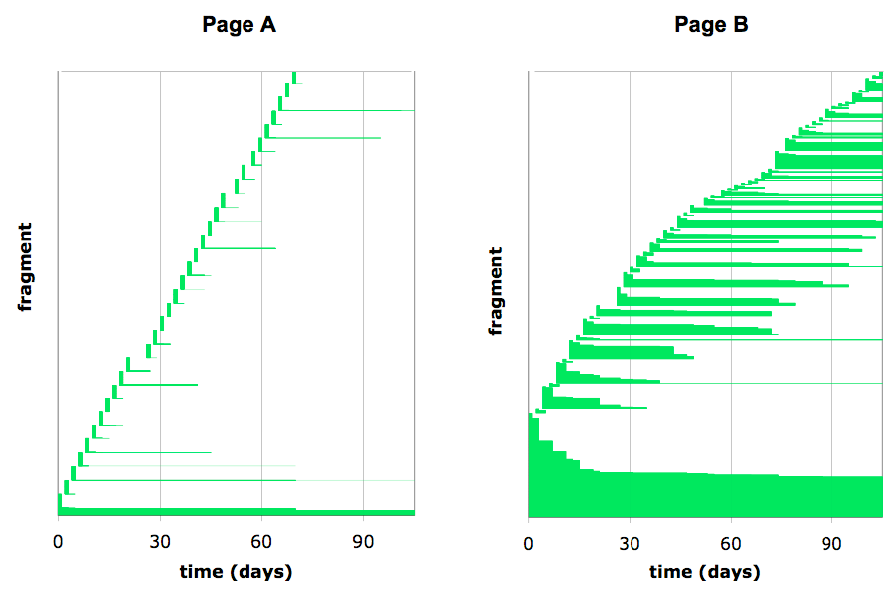
\includegraphics[width=65mm]{2008-Olston-recrawl.png}
%\caption{ Page A shows rapidly appearing and disappearing content, while Page B shows longer-lived content. This image was originally published in Olston's 2008 paper \cite{olston2008recrawl}.}
%\label{olston}
%\end{center}
%\end{figure}


Memento is a joint project between Old Dominion University and Los Alamos National Laboratory.  The Memento Framework defines HTTP extensions that allow content negotiation in the dimension of time \cite{nelson:memento:tr, ldow2010:memento}.  When used with Memento-aware user agents like MementoFox \cite{sandersonimplementing}, users can set a desired datetime in the past and browse the Web as it existed at (or near) that datetime.  Unlike other, single-archive applications like DiffIE \cite{Teevan:2010:LSH:1753326.1753530, 1622221}, Past Web Browser \cite{jatowt2006journey}, or Zoetrope \cite{adar2008zoetrope}, Memento provides an multi-archive approach to presenting the past Web. Integrating multiple Web archives can give a more complete picture of the past Web \cite{hmotwia}.

\section{Experiment design}
\label{experiment}
\vskip -3mm

%%%%TPDL 2013 ADDITION
SiteStory was tested with a variety of loads on a variety of resources. Three different tests were run during the experiment.

%%%%TPDL 2013 COMMENT
%SiteStory was tested with a variety of loads, a variety of resources, and on two machines with different configurations and specifications. Three different tests were run during the experiment. The details of the experiment setup and execution is included in this section.

\subsection{Experiment Machines}
\label{machines}
\vskip -3mm

The SiteStory benchmarking experiment was conducted with a pre-release
version of SiteStory installed on a machines referred to as PC1. PC1 has a single core 2.8 GHz processor, 
ran the prefork version of the Apache 2 Web server, and the mod\_sitestory-enabled Apache server provided content
from \url{localhost:8080}. The SiteStory archive was installed as a separate service at
\url{localhost:9999}.  Although the developers have experimented with optimizations
discussed in Section \ref{ta}, SiteStory currently archives all
returned representations regardless of whether the representation has
changed or not.


%%%%TPDL 2013 COMMENT
%PC1 has a single core 2.8 GHz processor.  It has no memory remaining
%on the server; it is 100\% utilized. PC1 represents a worst-case
%scenario for a server -- it has been completely bogged down with
%background processes. To simulate this load, a script runs throughout
%the experiment that initiates requests for Web pages to create the load
%on the server. PC1 ran Linux
%Ubuntu version 11. The results from the simulation are provided
%in Section \ref{results}.\\


\subsection{Experiment Runs}
\label{runs}
\vskip -3mm
Three separate experiments were run on PC1. The first experiment tests the throughput of a content server enabled with SiteStory software. The second experiment performs a series of accesses to 100 static resources to test the access rates, response times, and round trip times possible. The third experiment performs a series of accesses to 100 dynamic, constantly changing set of 100 resources to demonstrate a worst-case scenario for SiteStory -- everything is archived on each access. 

\subsection{Connection Handling: ab}
\label{ab}
\vskip -3mm
This first experiment to measure the differences in throughput when SiteStory is running and when SiteStory is turned off was run twice a day 
%(at 0700 and 1900 EST) 
for 45 days, resulting in 90 data points. 
%The experiment utilized the ab (ApacheBench) tool\footnote{\texttt{http://httpd.apache.org/docs/2.0/programs/ab.html}}. This utility makes N number of connections with C concurrency (meaning C connections are executing in parallel), where N and C are variables specified by the user.
The experiment uses the ab (ApacheBench) tool\footnote{\texttt{http://httpd.apache.org/docs/2.0/programs/ab.html}}, with a total of N
connections made with a concurrency of C connections, where N and C are
specified by the user.
 The ab utility records the response, throughput, and other server stats during a test. Essentially, the ApacheBench utility issues HTTP GET requests for content to establish a benchmark for performance. 
%A run in ab provides output similar to that seen in Appendix \ref{abApp}.

Three different HTML resources were targeted with this test: a small, medium, and large file of sizes 1kB, 250 kB, and 700 kB. 
%These resource sizes were chosen after a brief survey of the average file sizes in a corporate intranet provided a minimum, average, and maximum file size of a Web page\footnote{These file sizes were empirically determined in an internal MITRE study.}. 
We used combinations of N=(1,000, 10,000, 100,000, 216,000) and C=(1, 100, 200, 450) as parameters to the ab utility. 
%We chose the connection numbers of 1,000, 10,000, and 100,000 arbitrarily. 
%We chose the connection number of 216,000 after observing this as 2011's yearly maximum hourly rate of Website access\footnote{We chose this access rate after observing the average 2011 Website access rate within MITRE's corporate intranet.}. 
%Similarly, we chose the access concurrencies of 1, 100, and 200  arbitrarily, but we chose the concurrency of 450 as the observed average expected number of concurrent accesses to a site\footnote{We chose this access concurrency after observing the average 2011 Website access rate within MITRE's corporate intranet.}. 
We chose the file sizes, connection, and concurrency values to match the values observed in our study of MITRE's Corporate Intranet. 
For simplicity and brevity, this report discusses the runs of 10,000 connections with concurrencies 1 and 100, and runs of 216,000 connections with concurrencies 1 and 100. 
This subset of results illustrates typical results of all other tests. 

We modified the three resources between each set of connections to ensure the resource is archived each run. To modify the resources, we ran a script to update a timestamp displayed on each page and change the image that was embedded in the page. These modifications would ensure that not only the image was changed and able to be re-archived, but the surrounding HTML was changed, as well. Since SiteStory re-archives content whenever a change is detected, each test run results in each resource being re-archived. It is essential to make sure the resource is re-archived to observe the effect of an archival action on the content server performance.

We ran each ab test twice: once while SiteStory was turned on, and once while it was turned off. This shows how SiteStory affects the content server performance. A subset of the results are provided in Figure \ref{tares}. The red lines represent the runs in which SiteStory was turned off, while the blue lines represent the runs in which SiteStory was turned on. Each entry on the x-axis represents an independent test run. The y-axis provides the amount of time it took to execute the entire ab run. The horizontal lines represent the averages over the entire experiment. The dotted, vertical green lines indicate machine restart times due to power outages. The power outages were noted to show when a cache and memory resets may have occurred that could impact the performance of the machines.
 
To illustrate how SiteStory affects the content server's performance, please reference Figure \ref{tares} 
%and \ref{tares2}
that portrays the changes in the total run time of the ab test when SiteStory is on (actively archiving served content) and off (not archiving served content).

\begin{figure*}[ht!]
  \begin{center}
    \subfigure[Total run time for the ab test with 10,000 connections and 1 concurrency.]{\label{tr1}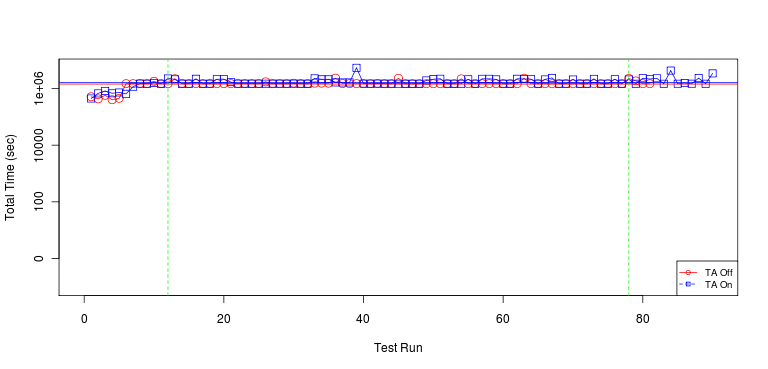
\includegraphics[width=1\textwidth]{totalRunTime2.png}} \\
    \subfigure[Total run time for the ab test with 10,000 connections and 100 concurrency.]{\label{tr2}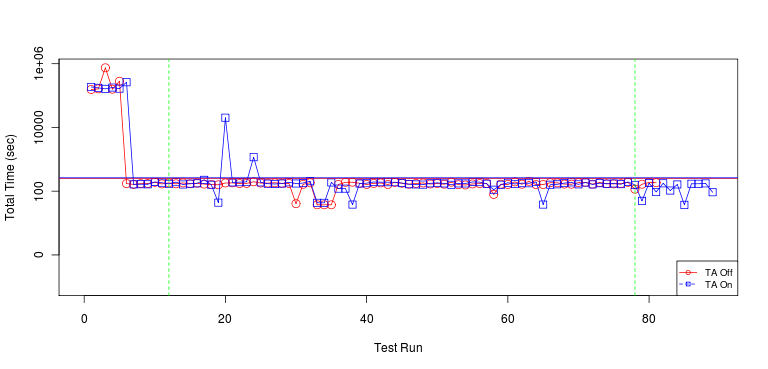
\includegraphics[width=1\textwidth]{totalRunTime1.png}} 
  \end{center}
  \caption{Total run time for 10,000 Connections.}
  \label{tares}
\end{figure*}


%\begin{figure*}[htp]
%  \begin{center}
%    \subfigure[Total run time for the ab test with 216,000 connections and 1 concurrency.]{\label{tr3}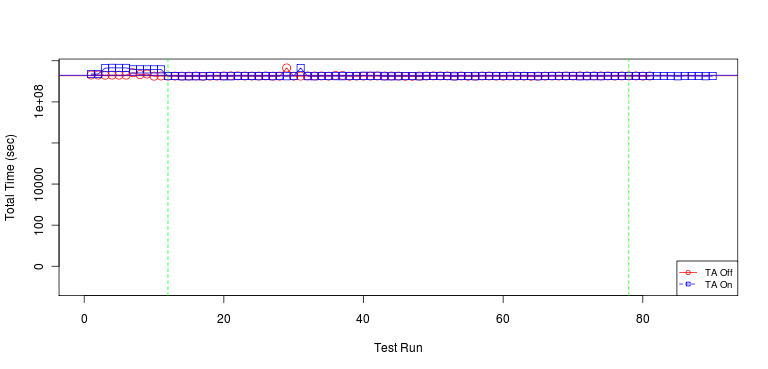
\includegraphics[width=1\textwidth]{totalRunTime4.png}} \\
%    \subfigure[Total run time for the ab test with 216,000 connections and 100 concurrency.]{\label{tr4}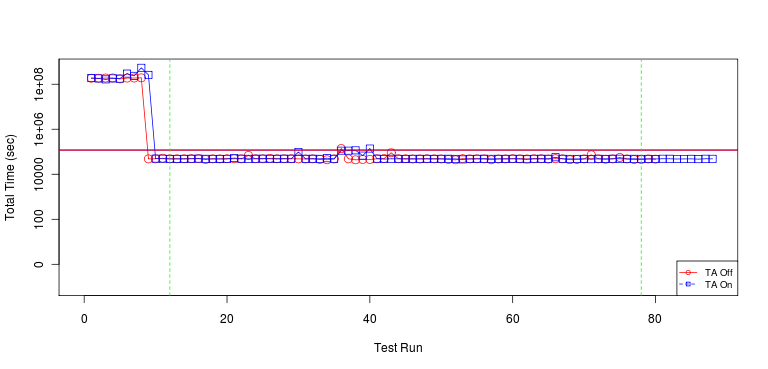
\includegraphics[width=1\textwidth]{totalRunTime3.png}} 
%  \end{center}
%  \caption{Total run time for 216,000 Connections.}
%  \label{tares2}
%\end{figure*}

\subsection{100 Static Resources: Clearing the Cache}
\label{static}
\vskip -3mm
The second experiment uses the \texttt{curl} command to access 100 different HTML resources, none of which change. After running the ab tests in Section \ref{ab}, a theory was formulated that a reason for some of the anomalies was from server caching.  This additional test shows the effect of clearing the server cache on SiteStory by accessing a large number of large files in sequence. This access essentially thrashes the server cache. Each resource has text, and between 0 and 99 images (the 0th resource has 0 images, the 1st resource has 1 image, etc.). These resources were generated by a Perl script that constructed 100 different HTML pages and embedded between 0-99 different images in the generated resources. The resources were created with different sizes, and different numbers of embedded resources to demonstrate how SiteStory affects content server performance with a variety of page sizes and embedded images.

%Figures \ref{pc100} and \ref{pc200} 
Figure \ref{pc100} demonstrates the accesses of the 100 resources. The dark blue and red lines indicate the average run time for accessing a resource (in seconds). The filled areas around the lines are the standard deviation ($\sigma$) of the observations over the duration of the experiment.



\begin{figure*}[ht!]
  \begin{center}
    \subfigure[Total access time for the 100 static resources on PC1.]{\label{ts1}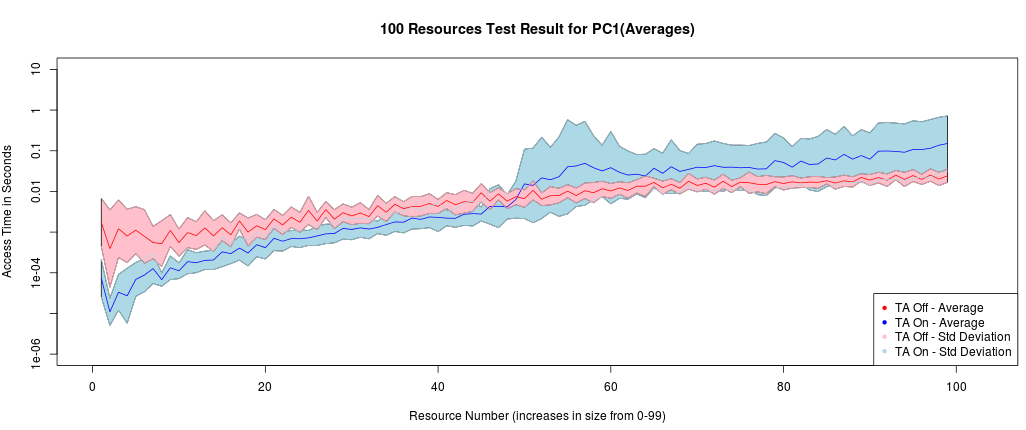
\includegraphics[width=1\textwidth]{loaded100testresults_pc1_sd_rev.png}} \\
    \subfigure[Total access time for the 100 changing resources on PC1.]{\label{tc1}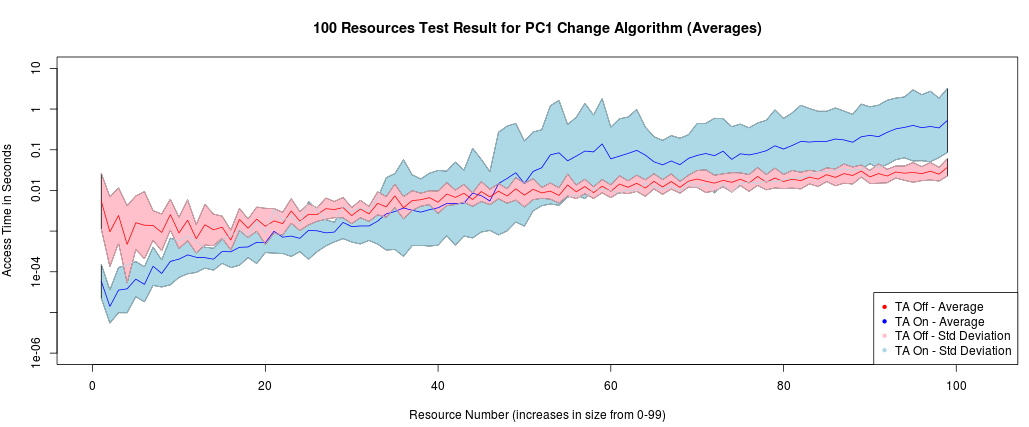
\includegraphics[width=1\textwidth]{loaded100testresults_pc1_change_sd_rev.png}} 
  \end{center}
  \caption{100 resources accessed on PC1. Resource \emph{n} has \emph{n} embedded images.
}
  \label{pc100}
\end{figure*}


%%%%TPDL 2013 COMMENT
%\begin{figure*}[htp]
%  \begin{center}
%    \subfigure[Total access time for the 100 static resources on PC2.]{\label{ts2}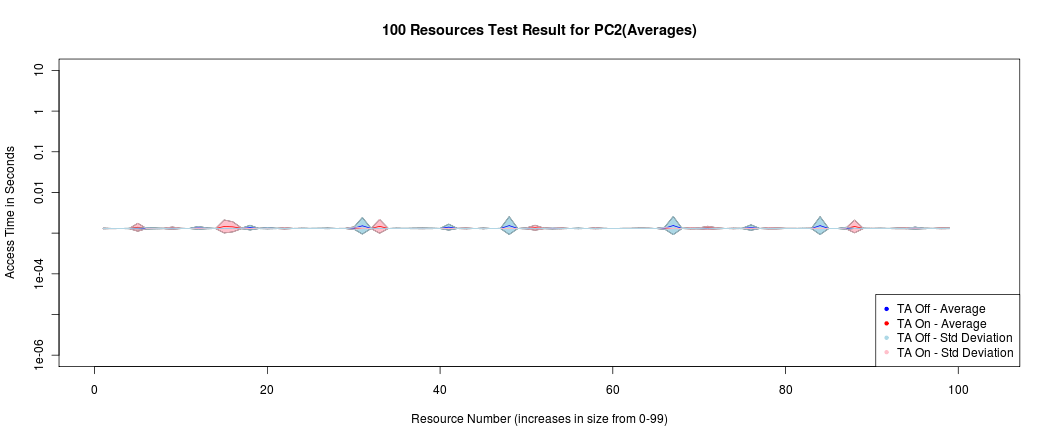
\includegraphics[width=150mm]{loaded100testresults_pc2_sd.png}} \\
%    \subfigure[Total access time for the 100 changing resources on PC2.]{\label{tc2}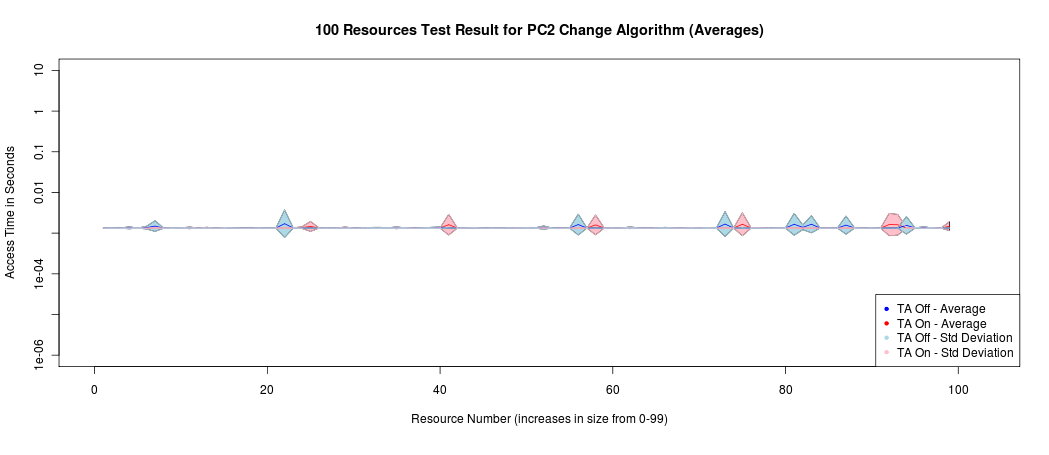
\includegraphics[width=150mm]{loaded100testresults_pc2_change_sd.png}} 
%  \end{center}
%  \caption{100 resources accessed on PC2. Resource \emph{n} has \emph{n} embedded images.}
%  \label{pc200}
%\end{figure*}



\subsection{100 Changing Resources: Worst-Case Scenario}
\label{changes}
\vskip -3mm
We ran the same experiment from Section \ref{static} in which each resource changes between runs to provide a ``worst case scenario'' of data connections vs. archiving and run time. We executed a script in between each run in which each resource was updated to make SiteStory archive a new copy of the resource. This means that each access resulted in a new archived copy of each resource. The results of this run are shown in Figure \ref{ts3}. 


Note that Figure \ref{pc1002} show a  ``burdened'' system. An artificial user load was induced on the servers to simulate a production environment in which many users are requesting content. A script was run during the test that made curl calls to the server pages to induce the load. Figure \ref{pc1002} shows the impact of SiteStory operating in a burdened environment. 


\begin{figure*}[ht!]
  \begin{center}
    \subfigure[Total access time for the 100 static resources on a burdened PC1.]{\label{ts3}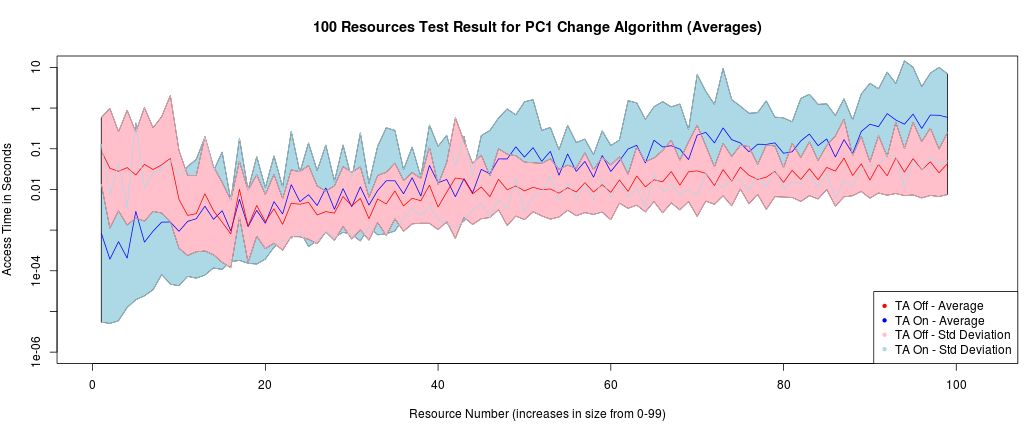
\includegraphics[width=1\textwidth]{unloaded100testresults_pc1_change_sd_rev.png}} \\
    \subfigure[Total access time for the 100 changing resources on a burdened PC1.]{\label{tc3}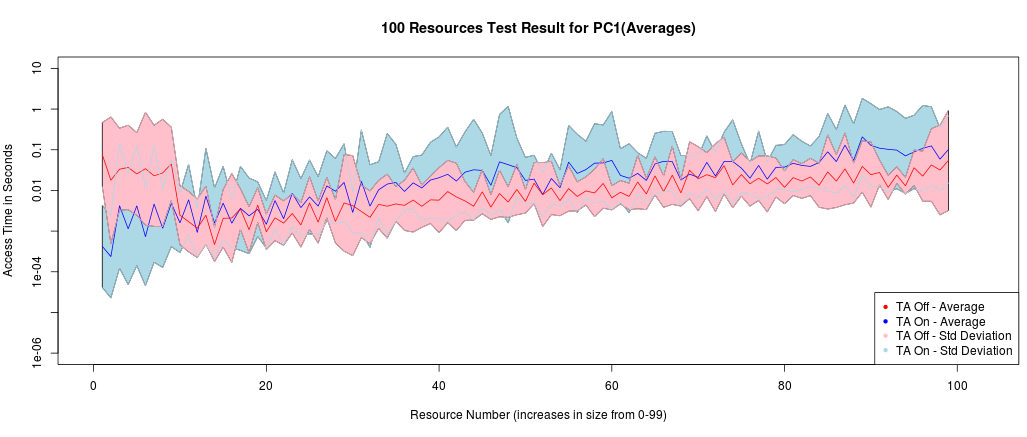
\includegraphics[width=1\textwidth]{unloaded100testresults_pc1_sd_rev.png}} 
  \end{center}
  \caption{100 resources accessed on a burdened PC1. Resource \emph{n} has \emph{n} embedded images.}
  \label{pc1002}
\end{figure*}



%%%%TPDL 2013 COMMENT
%\begin{figure*}[htp]
%  \begin{center}
%    \subfigure[Total access time for the 100 static resources on a burdened PC2.]{\label{ts4}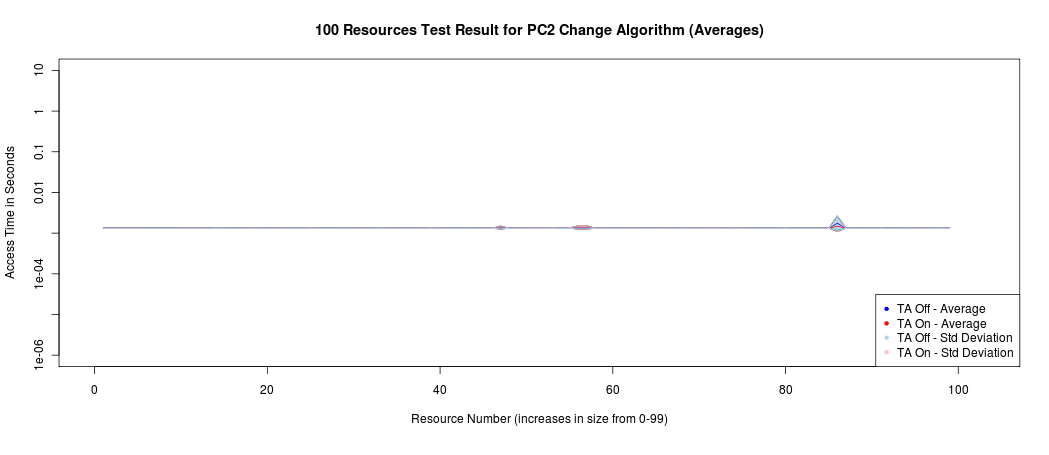
\includegraphics[width=150mm]{unloaded100testresults_pc2_change_sd.png}} \\
%    \subfigure[Total access time for the 100 changing resources on a burdened PC2.]{\label{tc4}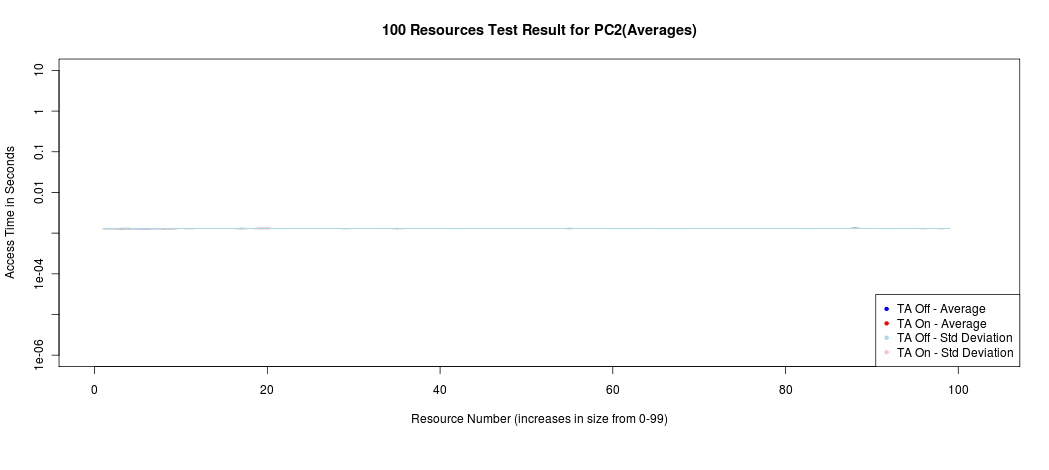
\includegraphics[width=150mm]{unloaded100testresults_pc2_sd.png}}
%  \end{center}
%  \caption{100 resources accessed on a burdened PC2. Resource \emph{n} has \emph{n} embedded images.}
%  \label{pc2002}
%\end{figure*}



\section{Results}
\label{results}
\vskip -3mm
%After the completion of the experiment, the results of each test were analyzed. Immediately, patterns emerge between graphs and tests demonstrating the effect of SiteStory on content server performance. 
This section explores the results of the tests, from which we conclude whether or not SiteStory affects its host content server in an acceptable manner. 

\subsection{ab Results}
\label{abresults}
\vskip -3mm
For the ApacheBench tests described in Section \ref{ab}, several obvious patterns emerge. Primarily, there is little separation between the total run times of the ab tests when SiteStory is on and when SiteStory is off. One can observe only minor differences in the plotted results. The results differ very little between any given run of the tests, and the averages across the experiment are almost identical in all tests. In the run of N=10,000 and C=1, the average total run times were 6.156 seconds when SiteStory was off, and 6.214 seconds when SiteStory was on.  In the run of N=10,000  and C=100, the average total run time was 2.4 seconds when SiteStory was off, and 2.42 seconds when SiteStory was on. In the run of N=216,000 and C=1, the average run time was 8.905 seconds when SiteStory was off, and 8.955 seconds when SiteStory was on. In the run of N=216,000 and C=100, the average total run time was 4.698 seconds when SiteStory was off, and the average total run time was 4.706 when SiteStory was on. This indicates SiteStory does not significantly affect the run time of the ab statistics, and therefore does not affect the performance of the content server with regard to content delivery time. 

Additionally, C=1 resulted in more consistent executions across each run whereas the runs with C=100 are more inconsistent, as indicated by the spikes in runtime. This could potentially be because of server caching, connection limitations, or even machine memory restrictions. The runs of C=100 also begin with a much longer total run time before dropping significantly and leveling out at runs 9 and 10. 
%The total run time with 10,000 connections was reduced from [INSERT NUMBER HERE] to [INSERT NUMBER HERE] around runs 9 and 10. The total run time with 216,000 connections was reduced from [INSERT NUMBER HERE] to [INSERT NUMBER HERE] around runs 9 and 10. 
This is due to additional processes running on the experiment machines that induced extra load in runs 1-8. However, the spikes and inconsistencies do not affect a single run, and do not affect only the runs in which SiteStory is on or those when SiteStory is off. As such, these anomalies are disregarded since they affect both runs.

Finally, the runs of 216,000 connections take much longer to complete than the runs of 10,000 connections -- specifically, 2.736 seconds longer, on average. This is intuitive since more connections should take longer to run. Additionally, the runs of C=1 take 3.9 seconds longer than the runs of C=100. By executing more connections in parallel, the total run time is intuitively shorter. 

The ab test provides evidence that SiteStory does not significantly affect server content delivery time. As such, a production server can implement SiteStory without users observing a noticeable difference in server performance. 

\subsection{100 Resource Results}
\label{staticresults}
\vskip -3mm
The runs of the 100 resources are more interesting, and provide a deeper insight into how SiteStory affects the server's performance than the ab test. This section examines the results of both the static and changing resource tests, as they provide interesting contrasts in performance. The results are listed in Table \ref{table100}.

%%%%TPDL 2013 COMMENT
%When comparing the unburdened and burdened results (such as Figure \ref{ts1} vs. Figure \ref{ts3}), it was observed that the average run times are 0.071 and 0.086 seconds higher when the server is under load and SiteStory is off and on, respectively. Additionally, $\sigma$ between the accesses is much greater; 0.1292 and 0.1767 greater when SiteStory is on and off, respectively, as indicated by the wider standard deviation shown on the Figures. 

When comparing the unchanging vs changing resources (such as Figure \ref{ts1} vs. \ref{tc1}), it is apparent that  $\sigma$ is, on average, two times higher for the changing resources than the unchanging resources. (The average $\sigma$ for unchanging resource is 0.0839 and 0.1680 for changing resources.) Additionally, the average access times when SiteStory is off remains approximately the same when the resources change or remain the same. The interesting result is that the average access time increases from 0.15 seconds per GET to 0.21 seconds per GET for the changing resources when SiteStory is on. This is intuitive considering SiteStory needs to re-archive the accessed content during an access when the resource changes. 


The most important observation in Figures \ref{ts1} and \ref{tc3} is that the run time of this test is approximately 0.5 seconds higher on average when SiteStory is on vs. when SiteStory is off. This number is reached by comparing the difference in average run time for each test when SiteStory is on vs. off. For each on-off pair, the average difference was taken to reach the approximate 0.5 second difference across all tests. That is, the difference between the average run times of the tests in Figures \ref{ts1} when SiteStory is running (red) vs when SiteStory is off (blue) is 0.08 seconds. When the same comparison is performed across all tests and the average of these results is taken, an overall impact of SiteStory on server performance is realized.

Each figure begins with SiteStory off taking more time than when SiteStory is on, but this can be attributed to experiment anomaly or similar server access anomaly. Inevitably, the run time when SiteStory is on becomes slower than when SiteStory is off as the resource size increases. This demonstrates that the performance difference of a server when SiteStory is on vs. off is worse when there is a large amount of embedded resources, such as images. PC1's average page access time increases by, on average, 0.006 seconds per embedded image. One could come to the conclusion that servers providing access to image-laden resources would see the biggest performance decrease when utilizing SiteStory. 

\begin{table*}[h!]
\caption{100 Resource Test Results} % title of Table
\centering % used for centering table
\begin{tabular}{c c c c c} % centered columns (4 columns)
\hline\hline %inserts double horizontal lines
Case & Avg. Unburdened & Unburdened $\sigma$ & Avg. Burdened & Burdened\\
     & Run Time & Unburdened $\sigma$ & Run Time  & Burdened $\sigma$\\ [0.5ex] % inserts table
%heading
\hline % inserts single horizontal line
\multicolumn{5}{c}{Static Resources}\\
\hline % inserts single horizontal line
SS Off & 0.121 & 0.0254 & 0.192 & 0.2021 \\
SS On & 0.206 & 0.1811 & 0.292 & 0.3103 \\
%PC2, SS Off & 0.056 & 0.0011 & 0.056 & 0.0001 \\
%PC2, SS On & 0.056 & 0.0009 & 0.056 & 0.0001 \\
\hline \hline
\multicolumn{5}{c}{Changing Resources}\\
\hline % inserts single horizontal line
SS Off & 0.132 & 0.0346 & 0.225 & 0.2174 \\
SS On & 0.354 & 0.4244 & 0.292 & 0.6137 \\
%PC2, SS Off & 0.057 & 0.0021 & 0.056 & 0.0002 \\
%PC2, SS On & 0.057 & 0.0016 & 0.056 & 0.0002   \\ [1ex] % [1ex] adds vertical space
\hline %inserts single line
\end{tabular}
\label{table100} % is used to refer this table in the text
\end{table*}


\section{Conclusions}
\label{conclusion}
\vskip -3mm
%%mention that SiteStory does not significantly affect server performance (only slightly increases response time). 
In this work, we stress tested and benchmarked a pre-release version of SiteStory with the ApacheBench (ab) utility. Our experiment environment replicates resource sizes and access loads observed in  MITRE's Corporate Intranet. The results of this study show that SiteStory does not significantly affect the performance of a server. While different servers and different use cases cause different performance effects when SiteStory is archiving content, the host server is still able to serve sites in a timely manner. The type of resource and resource change rate also affects the server's performance -- resources with many embedded images and frequently changing content are affected most by SiteStory, seeing the biggest reduction in performance. 
%Additionally, through the case study of a corporate intranet, this solution has been shown to effectively archive content served to users. 

SiteStory does not significantly increase the load on a server or affect its ability to serve content -- the response times seen by users will not be noticeably different in most cases. However, these graphs demonstrate the impact of SiteStory on performance, albeit small -- larger resources with many embedded resources take longer to serve when SiteStory is on as opposed to when SiteStory is off due to the increased processing required of the server. However, the significant finding of this work is that SiteStory will not cripple, or even significantly reduce, a server's ability to provide content to users. Specifically, SiteStory only increases response times by a fraction of a second -- from 0.076 seconds to 0.086 seconds per access when the server is under load, and from 0.15 seconds to 0.21 seconds when the resource has many embedded and changing resources. These increases will not be noticed by human users.

%ACKNOWLEDGMENTS are optional

\section{Acknowledgments}
\vskip -3mm
This work is supported in part by NSF grant 1009392 and the Library of Congress. A Corporate Case Study to investigate the feasibility of a transactional archive in a corporate intranet was funded by a Fiscal Year 2011 Innovation Grant from the MITRE Corporation. MITRE employees Jory T. Morrison and George Despres were integral to the MITRE Innovation Grant and Case Study.

%Special thanks to Lyudmila Balakireva, Harihar Shankar, Martin Klein, Robert Sanderson and Herbert Van de Sompel from LANL for the design and development of SiteStory, and their feedback and guidance throughout this experiment. 


%\bibliographystyle{abbrv}
%\vskip -3mm
%\bibliography{_mybibtex}
\begin{thebibliography}{10}

\bibitem{adar2008zoetrope}
E.~Adar, M.~Dontcheva, J.~Fogarty, and D.~Weld.
\newblock {Zoetrope: interacting with the ephemeral web}.
\newblock In {\em Proceedings of the 21st annual ACM symposium on User
  interface software and technology}, pages 239--248. ACM, 2008.

\bibitem{hmotwia}
S.~Ainsworth, A.~Alsum, H.~SalahEldeen, M.~C. Weigle, and M.~L. Nelson.
\newblock {How much of the Web is archived?}
\newblock In {\em {JCDL '11: Proceedings of the 11th annual international
  ACM/IEEE Joint Conference on Digital Libraries}}, pages 133--136, 2011.

\bibitem{brewington2000keeping}
B.~Brewington, G.~Cybenko, D.~Coll, and N.~Hanover.
\newblock {Keeping up with the changing Web}.
\newblock {\em IEEE Computer}, 33(5):52--58, 2000.

\bibitem{cho2000evolution}
J.~Cho and H.~Garcia-Molina.
\newblock {The evolution of the web and implications for an incremental
  crawler}.
\newblock In {\em Proceedings of the 26th international conference on very
  large data bases}, pages 200--209, 2000.

\bibitem{Dyreson:2004:MVW:988672.988730}
C.~E. Dyreson, H.-l. Lin, and Y.~Wang.
\newblock {Managing versions of Web documents in a transaction-time Web
  server}.
\newblock In {\em Proceedings of the 13th international conference on World
  Wide Web}, WWW '04, 2004.

\bibitem{fetterly2004large}
D.~Fetterly, M.~Manasse, M.~Najork, and J.~Wiener.
\newblock {A large-scale study of the evolution of web pages}.
\newblock {\em Software: Practice and Experience}, 34(2):213--237, 2004.

\bibitem{transarch}
K.~Fitch.
\newblock {Web site archiving: an approach to recording every materially
  different response produced by a Website}.
\newblock In {\em {9th Australasian World Wide Web Conference}}, pages 5--9,
  July 2003.

\bibitem{hiddenurls}
K.~Hagedorn and J.~Sentelli.
\newblock {Google Still Not Indexing Hidden Web URLs}.
\newblock {\em D-Lib Magazine}, 14(7), August 2008.
\newblock \url{http://dlib.org/dlib/july08/hagedorn/07hagedorn.html}.

\bibitem{jatowt2006journey}
A.~Jatowt, Y.~Kawai, S.~Nakamura, Y.~Kidawara, and K.~Tanaka.
\newblock {Journey to the past: proposal of a framework for past web browser}.
\newblock In {\em Proceedings of the seventeenth conference on Hypertext and
  hypermedia}, pages 135--144. ACM, 2006.

\bibitem{olston2008recrawl}
C.~Olston and S.~Pandey.
\newblock {Recrawl scheduling based on information longevity}.
\newblock In {\em Proceeding of the 17th international conference on World Wide
  Web}, pages 437--446. ACM, 2008.

\bibitem{sandersonimplementing}
R.~Sanderson, H.~Shankar, S.~Ainsworth, F.~McCown, and S.~Adams.
\newblock {Implementing Time Travel for the Web}.
\newblock {\em Code4Lib Journal}, 13, 2011.

\bibitem{Teevan:2010:LSH:1753326.1753530}
J.~Teevan, S.~T. Dumais, and D.~J. Liebling.
\newblock A longitudinal study of how highlighting web content change affects
  people's web interactions.
\newblock In {\em Proceedings of the 28th international conference on Human
  factors in computing systems}, CHI '10, 2010.

\bibitem{1622221}
J.~Teevan, S.~T. Dumais, D.~J. Liebling, and R.~L. Hughes.
\newblock Changing how people view changes on the web.
\newblock In {\em UIST '09: Proceedings of the 22nd annual ACM symposium on
  User interface software and technology}, pages 237--246, 2009.

\bibitem{memento:rfc}
H.~{Van de Sompel}, M.~L. Nelson, and R.~Sanderson.
\newblock {HTTP framework for time-based access to resource states -- Memento
  draft-vandesompel-memento-06}.
\newblock \url{http://tools.ietf.org/pdf/draft-vandesompel-memento-06.pdf},
  2013.

\bibitem{nelson:memento:tr}
H.~{Van de Sompel}, M.~L. Nelson, R.~Sanderson, L.~L. Balakireva, S.~Ainsworth,
  and H.~Shankar.
\newblock {Memento: Time Travel for the Web}.
\newblock Technical Report arXiv:0911.1112, 2009.

\bibitem{ldow2010:memento}
H.~{Van de Sompel}, R.~Sanderson, M.~L. Nelson, L.~L. Balakireva, H.~Shankar,
  and S.~Ainsworth.
\newblock {An HTTP-Based Versioning Mechanism for Linked Data}.
\newblock In {\em Proceedings of the Linked Data on the Web Workshop (LDOW
  2010)}, 2010.
\newblock (Also available as arXiv:1003.3661).

\bibitem{511465}
J.~L. Wolf, M.~S. Squillante, P.~S. Yu, J.~Sethuraman, and L.~Ozsen.
\newblock {Optimal crawling strategies for web search engines}.
\newblock In {\em WWW '02: Proceedings of the 11th international conference on
  World Wide Web}, pages 136--147, 2002.

\end{thebibliography}

\end{document}
